\documentclass[11pt, a4paper]{article}
\usepackage{pdfpages}
\usepackage{parallel}
\usepackage[T2A]{fontenc}
\usepackage{ucs}
\usepackage[utf8x]{inputenc}
\usepackage[polish,english,russian]{babel}
\usepackage{hyperref}
\usepackage{rotating}
\usepackage[inner=2cm,top=1.8cm,outer=2cm,bottom=2.3cm,nohead]{geometry}
\usepackage{listings}
\usepackage{graphicx}
\usepackage{wrapfig}
\usepackage{longtable}
\usepackage{indentfirst}
\usepackage{array}
\usepackage{tikzsymbols}
\usepackage{soul}
\usepackage[ruled,vlined]{algorithm2e}
%\counterwithout{figure}{section} 

\usepackage{url}
\makeatletter
\g@addto@macro{\UrlBreaks}{\UrlOrds}
\makeatother

\newcolumntype{P}[1]{>{\raggedright\arraybackslash}p{#1}}
\frenchspacing
\usepackage{fixltx2e} %text sub- and superscripts
\usepackage{icomma} % коскі ў матэматычным рэжыме
\PreloadUnicodePage{4}

\newcommand{\longpage}{\enlargethispage{\baselineskip}}
\newcommand{\shortpage}{\enlargethispage{-\baselineskip}}

\def\switchlang#1{\expandafter\csname switchlang#1\endcsname}
\def\switchlangbe{
\let\saverefname=\refname%
\def\refname{Літаратура}%
\def\figurename{Іл.}%
}
\def\switchlangen{
\let\saverefname=\refname%
\def\refname{References}%
\def\figurename{Fig.}%
}
\def\switchlangru{
\let\saverefname=\refname%
\let\savefigurename=\figurename%
\def\refname{Литература}%
\def\figurename{Рис.}%
}

\hyphenation{admi-ni-stra-tive}
\hyphenation{ex-pe-ri-ence}
\hyphenation{fle-xi-bi-li-ty}
\hyphenation{Py-thon}
\hyphenation{ma-the-ma-ti-cal}
\hyphenation{re-ported}
\hyphenation{imp-le-menta-tions}
\hyphenation{pro-vides}
\hyphenation{en-gi-neering}
\hyphenation{com-pa-ti-bi-li-ty}
\hyphenation{im-pos-sible}
\hyphenation{desk-top}
\hyphenation{elec-tro-nic}
\hyphenation{com-pa-ny}
\hyphenation{de-ve-lop-ment}
\hyphenation{de-ve-loping}
\hyphenation{de-ve-lop}
\hyphenation{da-ta-ba-se}
\hyphenation{plat-forms}
\hyphenation{or-ga-ni-za-tion}
\hyphenation{pro-gramming}
\hyphenation{in-stru-ments}
\hyphenation{Li-nux}
\hyphenation{sour-ce}
\hyphenation{en-vi-ron-ment}
\hyphenation{Te-le-pathy}
\hyphenation{Li-nux-ov-ka}
\hyphenation{Open-BSD}
\hyphenation{Free-BSD}
\hyphenation{men-ti-on-ed}
\hyphenation{app-li-ca-tion}

\def\progref!#1!{\texttt{#1}}
\renewcommand{\arraystretch}{2} %Іначай формулы ў матрыцы зліпаюцца з лініямі
\usepackage{array}

\def\interview #1 (#2), #3, #4, #5\par{

\section[#1, #3, #4]{#1 -- #3, #4}
\def\qname{LVEE}
\def\aname{#1}
\def\q ##1\par{{\noindent \bf \qname: ##1 }\par}
\def\a{{\noindent \bf \aname: } \def\qname{L}\def\aname{#2}}
}

\def\interview* #1 (#2), #3, #4, #5\par{

\section*{#1\\{\small\rm #3, #4. #5}}
\ifx\ParallelWhichBox\undefined%
    \addcontentsline{toc}{section}{#1, #3, #4}%
\else%
\ifnum\ParallelWhichBox=0%
    \addcontentsline{toc}{section}{#1, #3, #4}%
\fi\fi%

\def\qname{LVEE}
\def\aname{#1}
\def\q ##1\par{{\noindent \bf \qname: ##1 }\par}
\def\a{{\noindent \bf \aname: } \def\qname{L}\def\aname{#2}}
}

\newcommand{\interviewfooter}[1]{
\vskip 1em
\noindent \textit{#1}
}

\switchlang{ru}
\begin{document}

\title{1996 "--- Hi-Bon Optical laser mouse LMOX-2}
\date{}
\maketitle
\selectlanguage{russian}
    Hi-Bon Optical laser mouse LMOX-2 (рис. \ref{fig:OpticalLaserMousePic}) выпускалась в Южной Корее и была, наряду с мышью Q500, одной из двух необычных оптических мышей, разработанных в 1996 году iO TEK и использующих в своей конструкции световоды. Разрешающая способность данной мыши составляет 450 точек на дюйм, а надпись на коробке помимо этого факта упоминает в качестве революционной особенности отсутствие шара и, соответственно, отсутствие необходимости в чистке.

\begin{figure}[h]
    \centering
    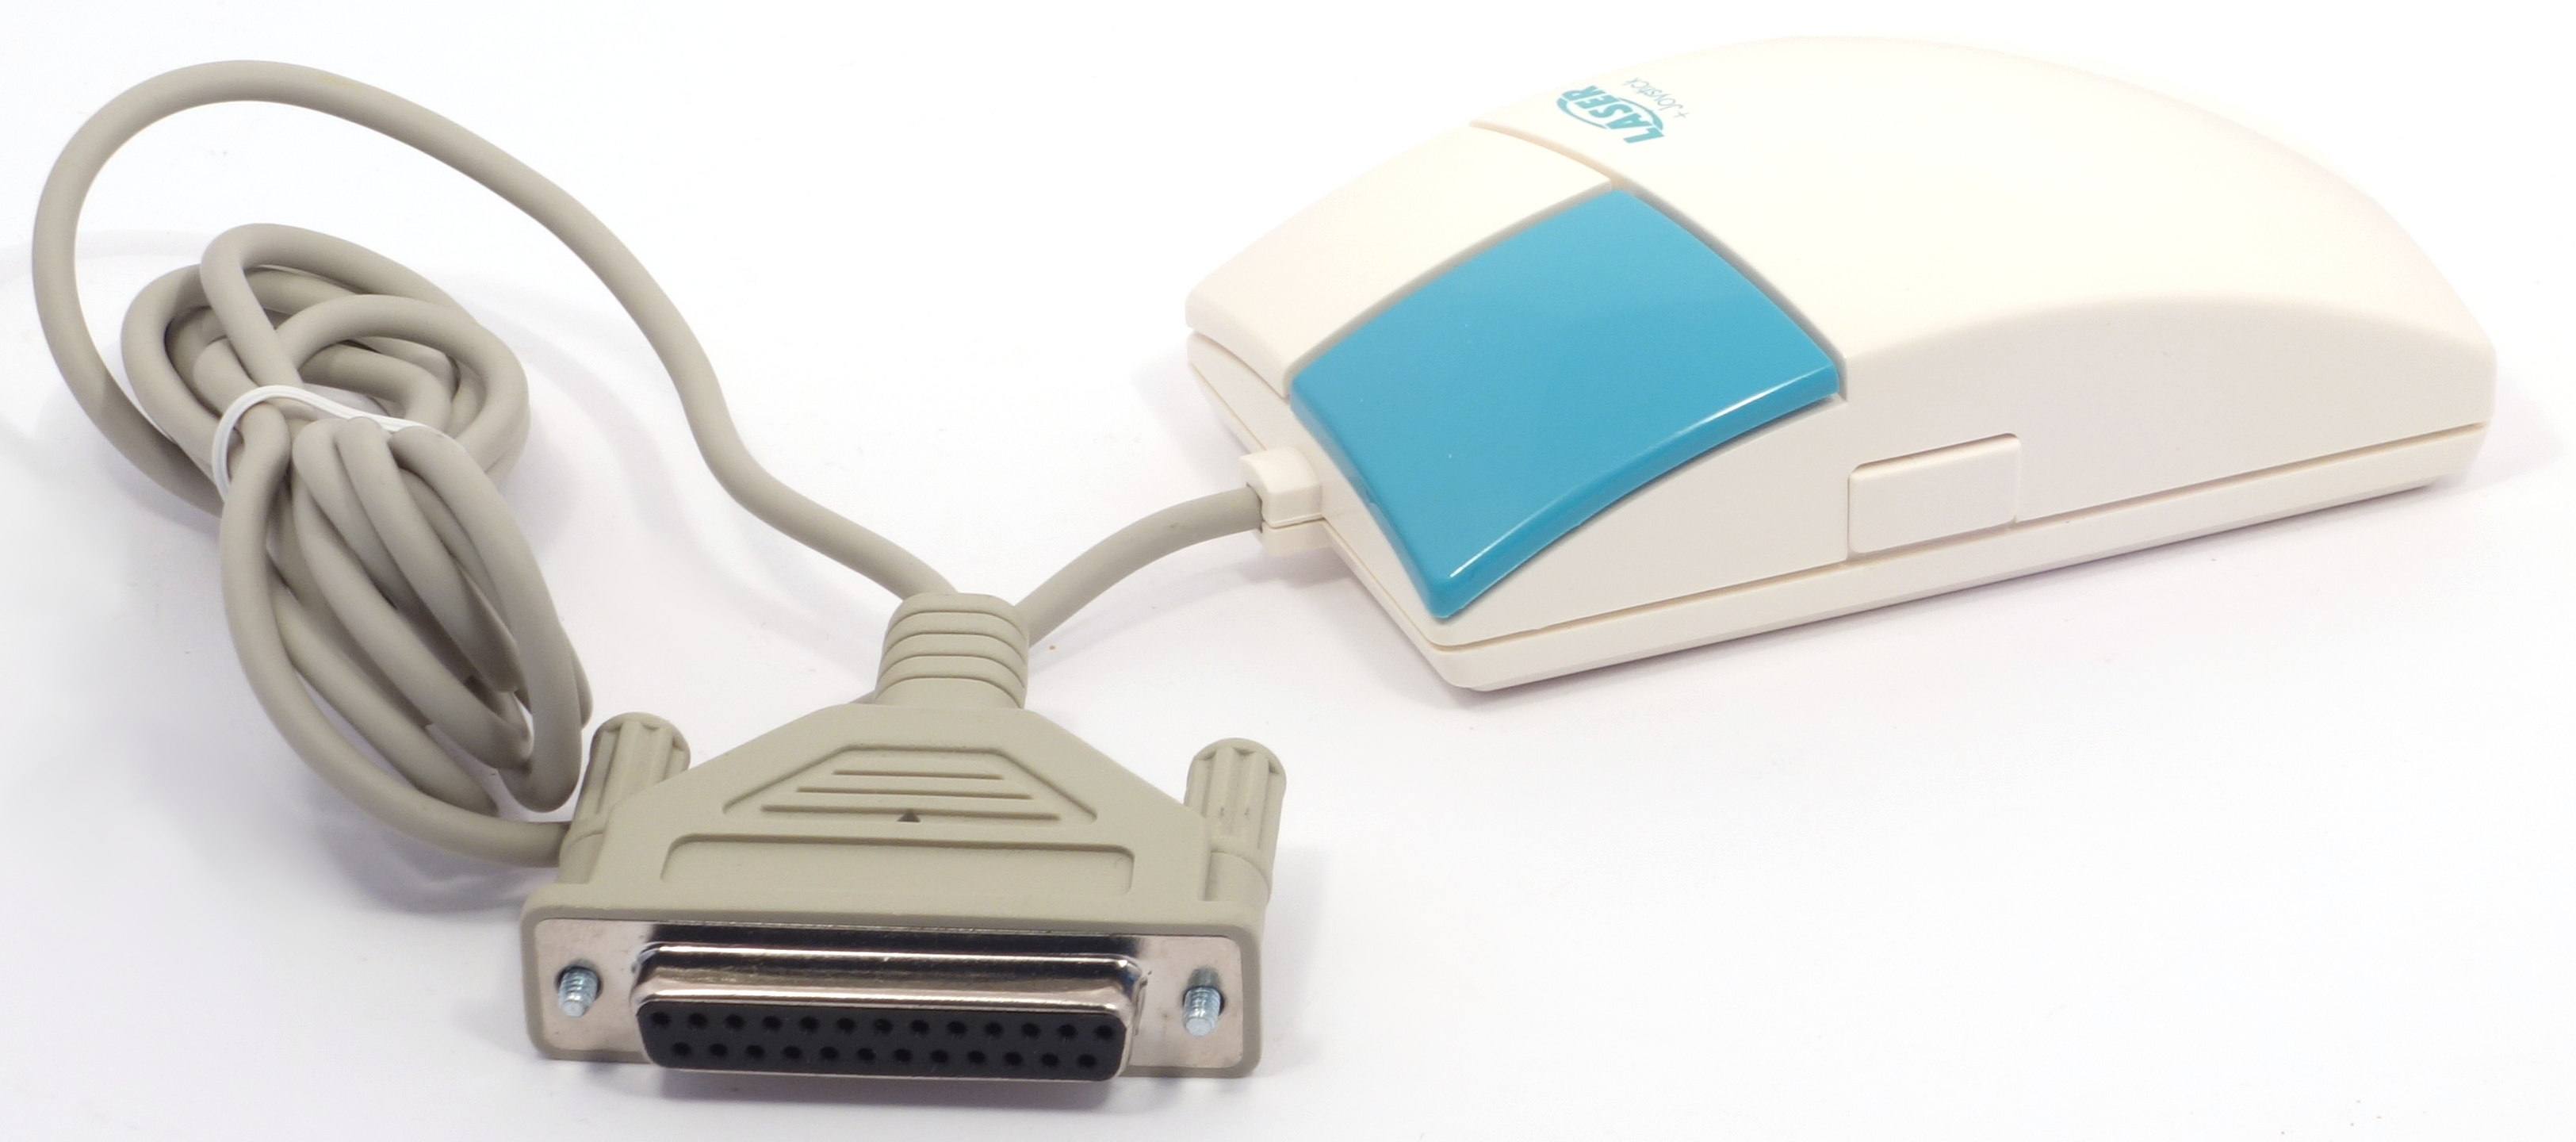
\includegraphics[scale=0.4]{1996_hi-bon_laser_mouse/pic_30.jpg}
    \caption{Hi-Bon Optical laser mouse}
    \label{fig:OpticalLaserMousePic}
\end{figure}

Как в случае абсолютного большинства ранних оптических мышей, данному манипулятору требуется коврик с отражающей сеткой (рис. \ref{fig:OpticalLaserMousePad}). В отличие от металлических ковриков Mouse Systems, здесь применяется белая поверхность, отражающая инфракрасное излучение, с нанесенными на нее черными точками, имеющими меньший коэффициент отражения в инфракрасном диапазоне. Коврик имеет небольшой размер, который однако компенсируется высокой разрешающей способностью мыши.

\begin{figure}[h]
    \centering
    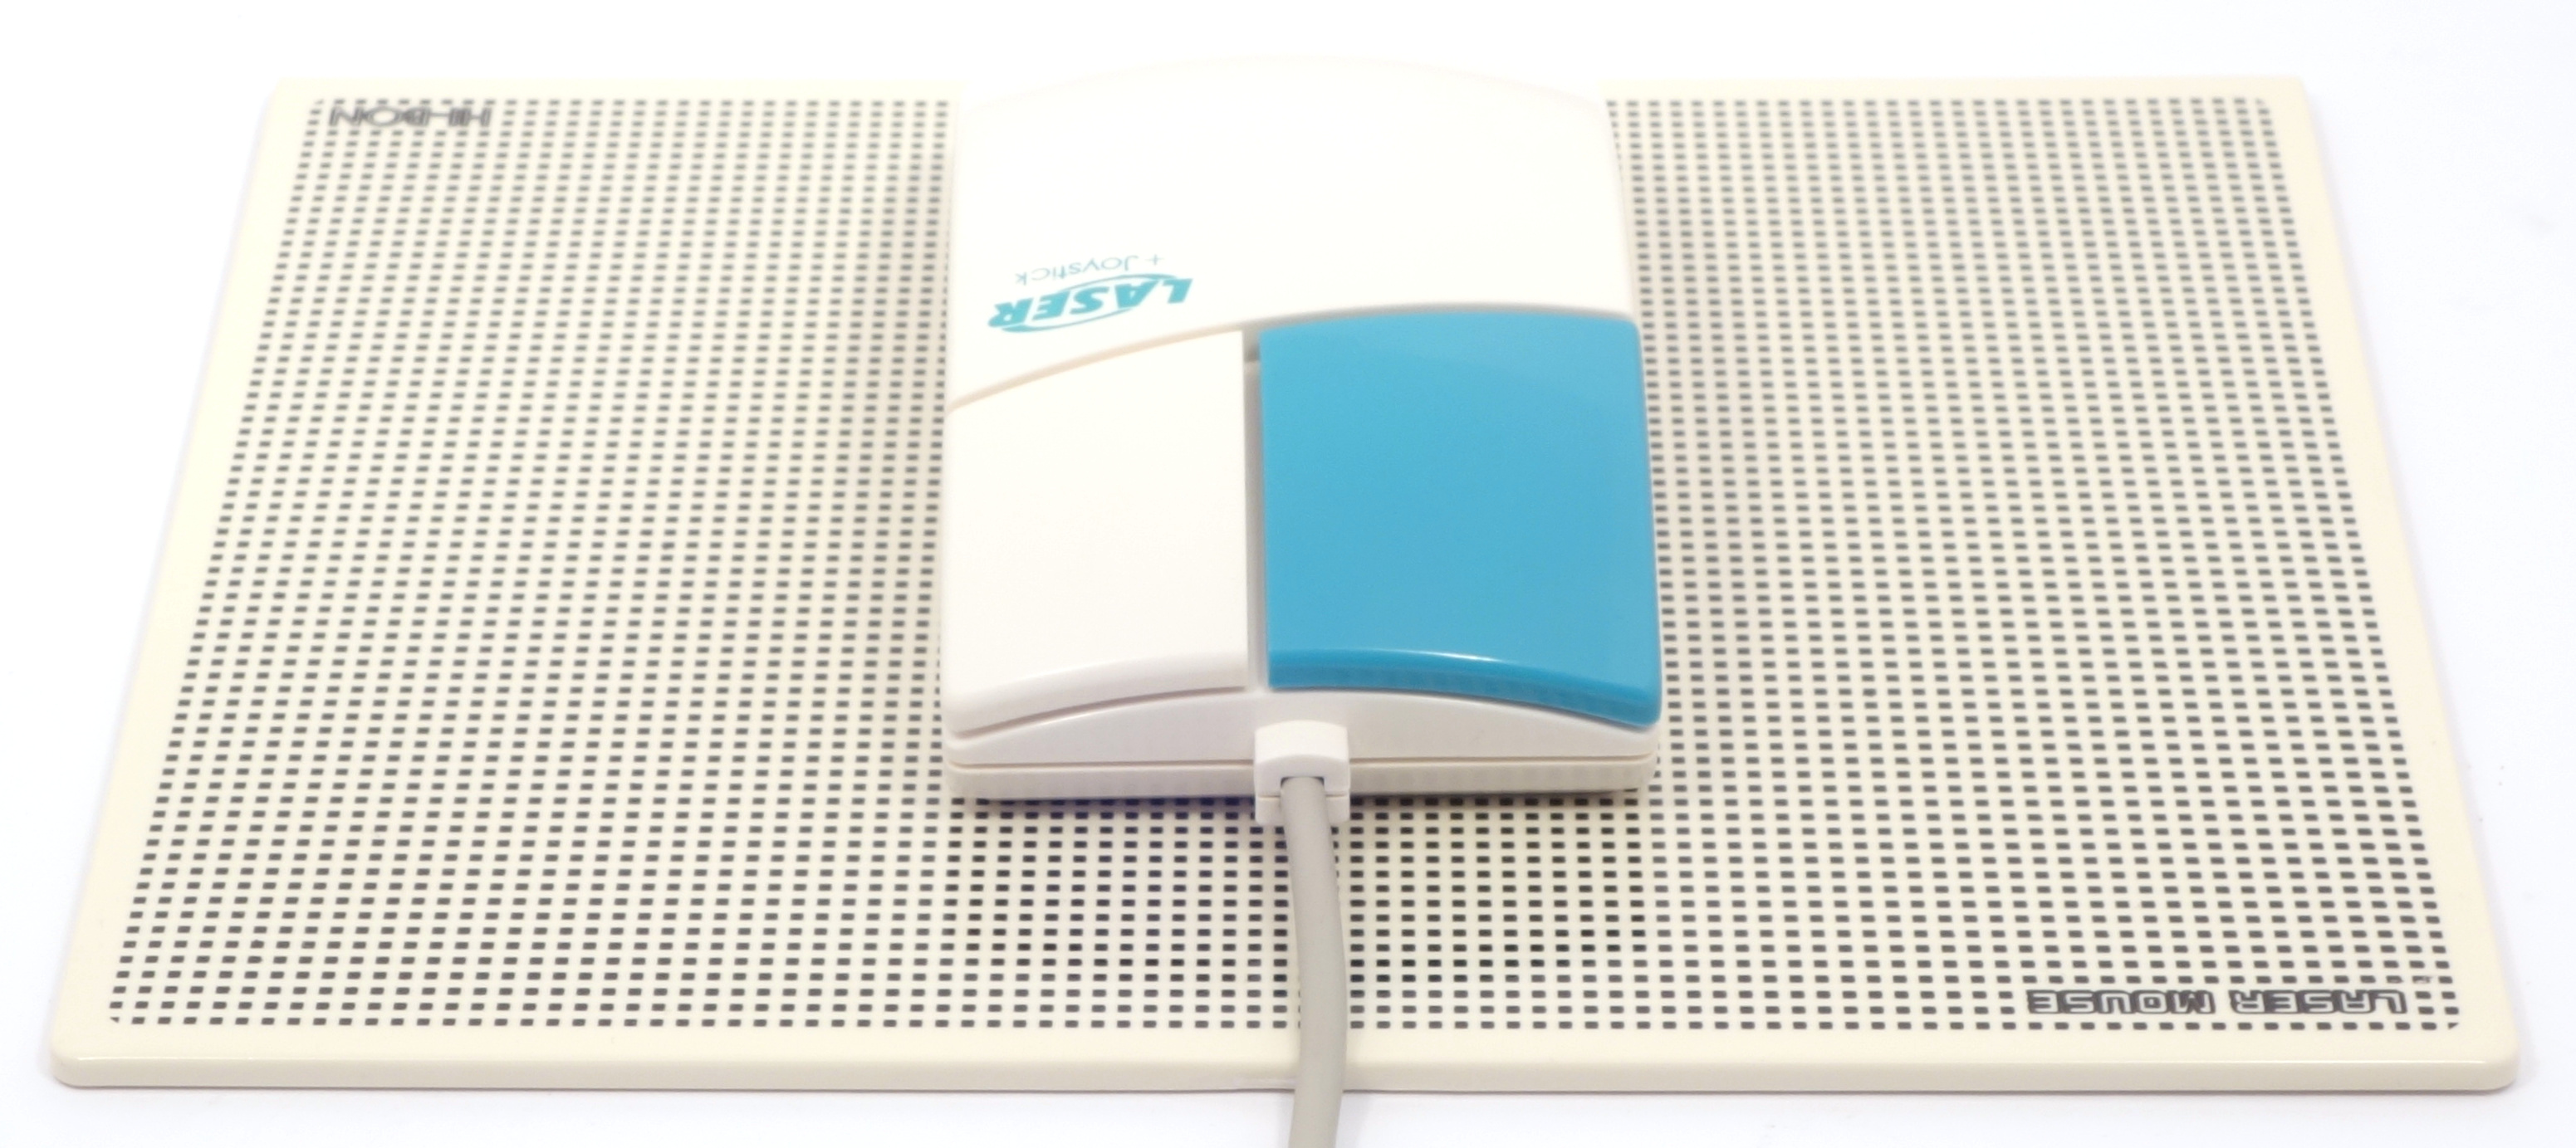
\includegraphics[scale=0.4]{1996_hi-bon_laser_mouse/pic2_30.jpg}
    \caption{Hi-Bon Optical laser mouse на комплектном коврике}
    \label{fig:OpticalLaserMousePad}
\end{figure}

Мышь имеет минималистичный дизайн и две кнопки, одна из которых выделена цветом (во второй половине 90-х это скорее дизайнерское решение, чем попытка наглядно показать пользователю главную кнопку мыши). С нижней стороны видны два светодиода и выходы 16 световодов (рис. \ref{fig:OpticalLaserMouseTopBottom}).

\begin{figure}[h]
    \centering
    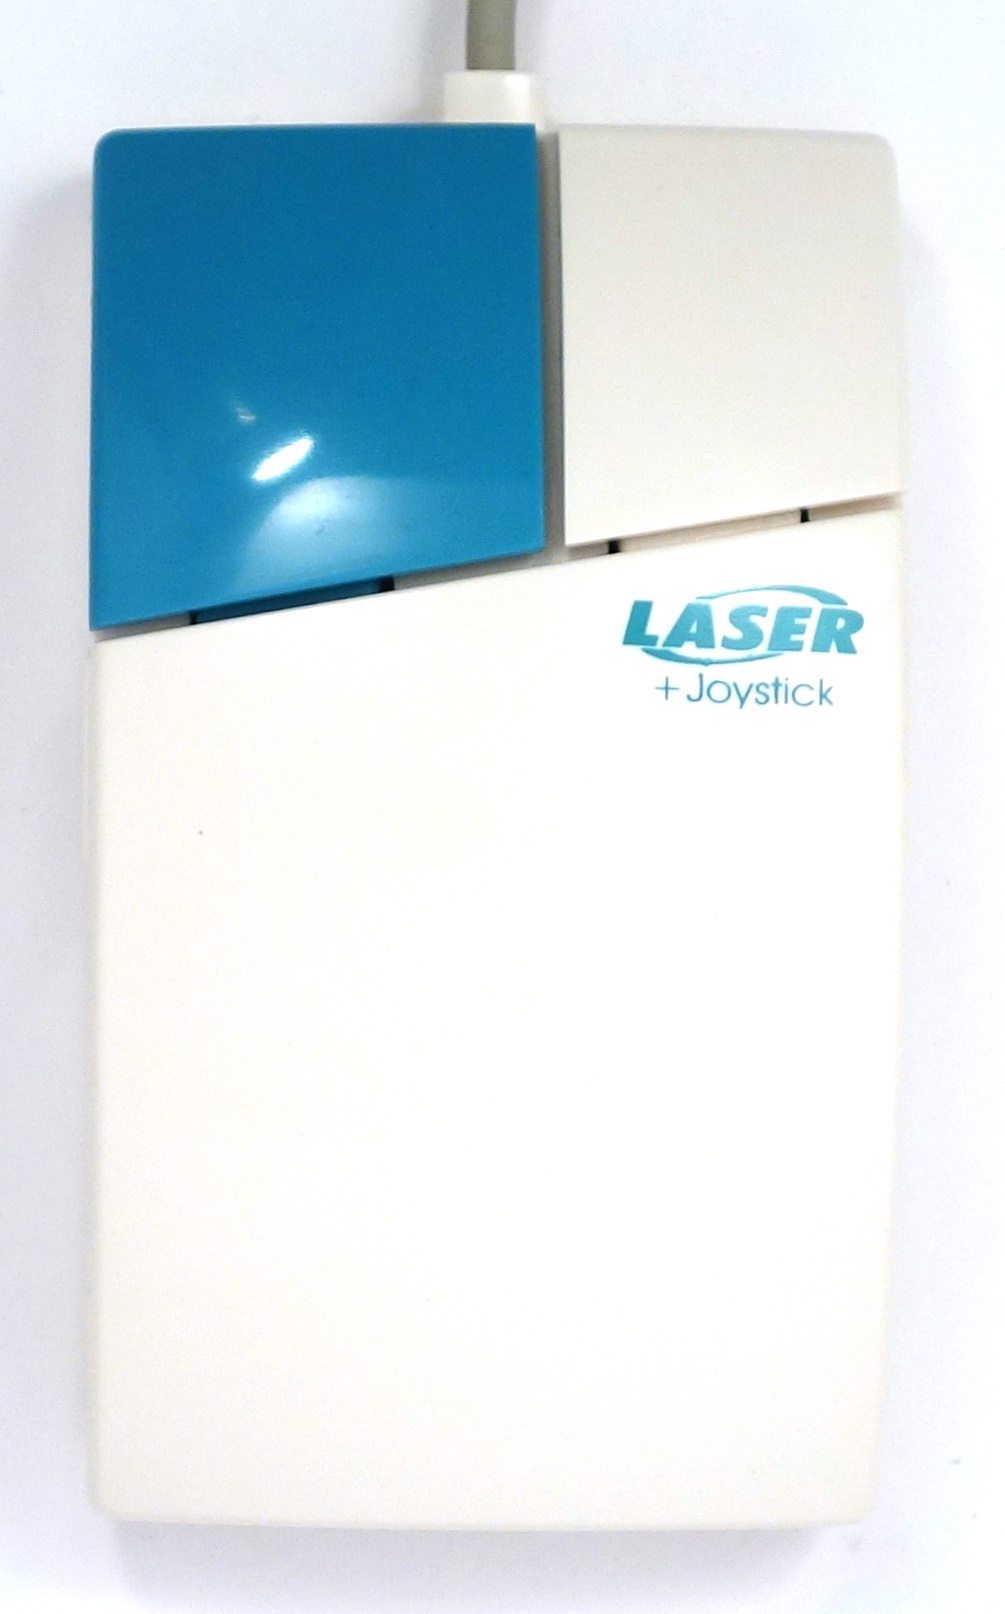
\includegraphics[scale=0.4]{1996_hi-bon_laser_mouse/top_60.jpg}
    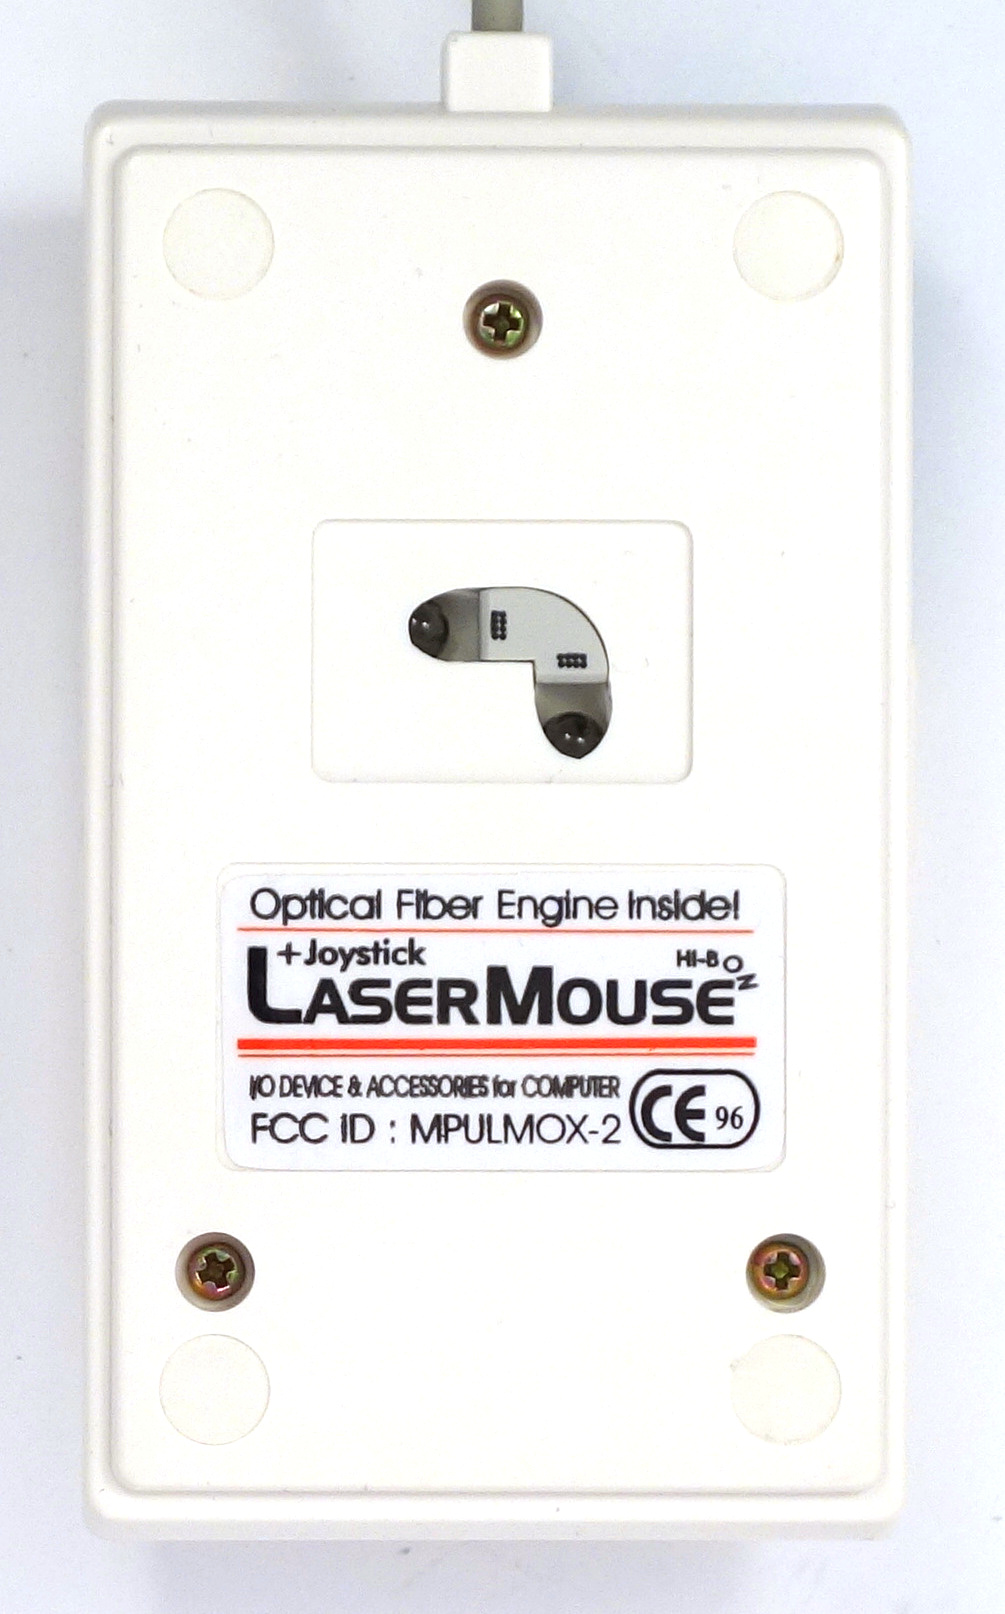
\includegraphics[scale=0.4]{1996_hi-bon_laser_mouse/bottom_60.jpg}
    \caption{Hi-Bon Optical laser mouse вид сверху и снизу}
    \label{fig:OpticalLaserMouseTopBottom}
\end{figure}

По размеру и форме мышь является типичным двухкнопочным манипулятором (рис. \ref{fig:OpticalLaserMouseSize}).

\begin{figure}[h]
    \centering
    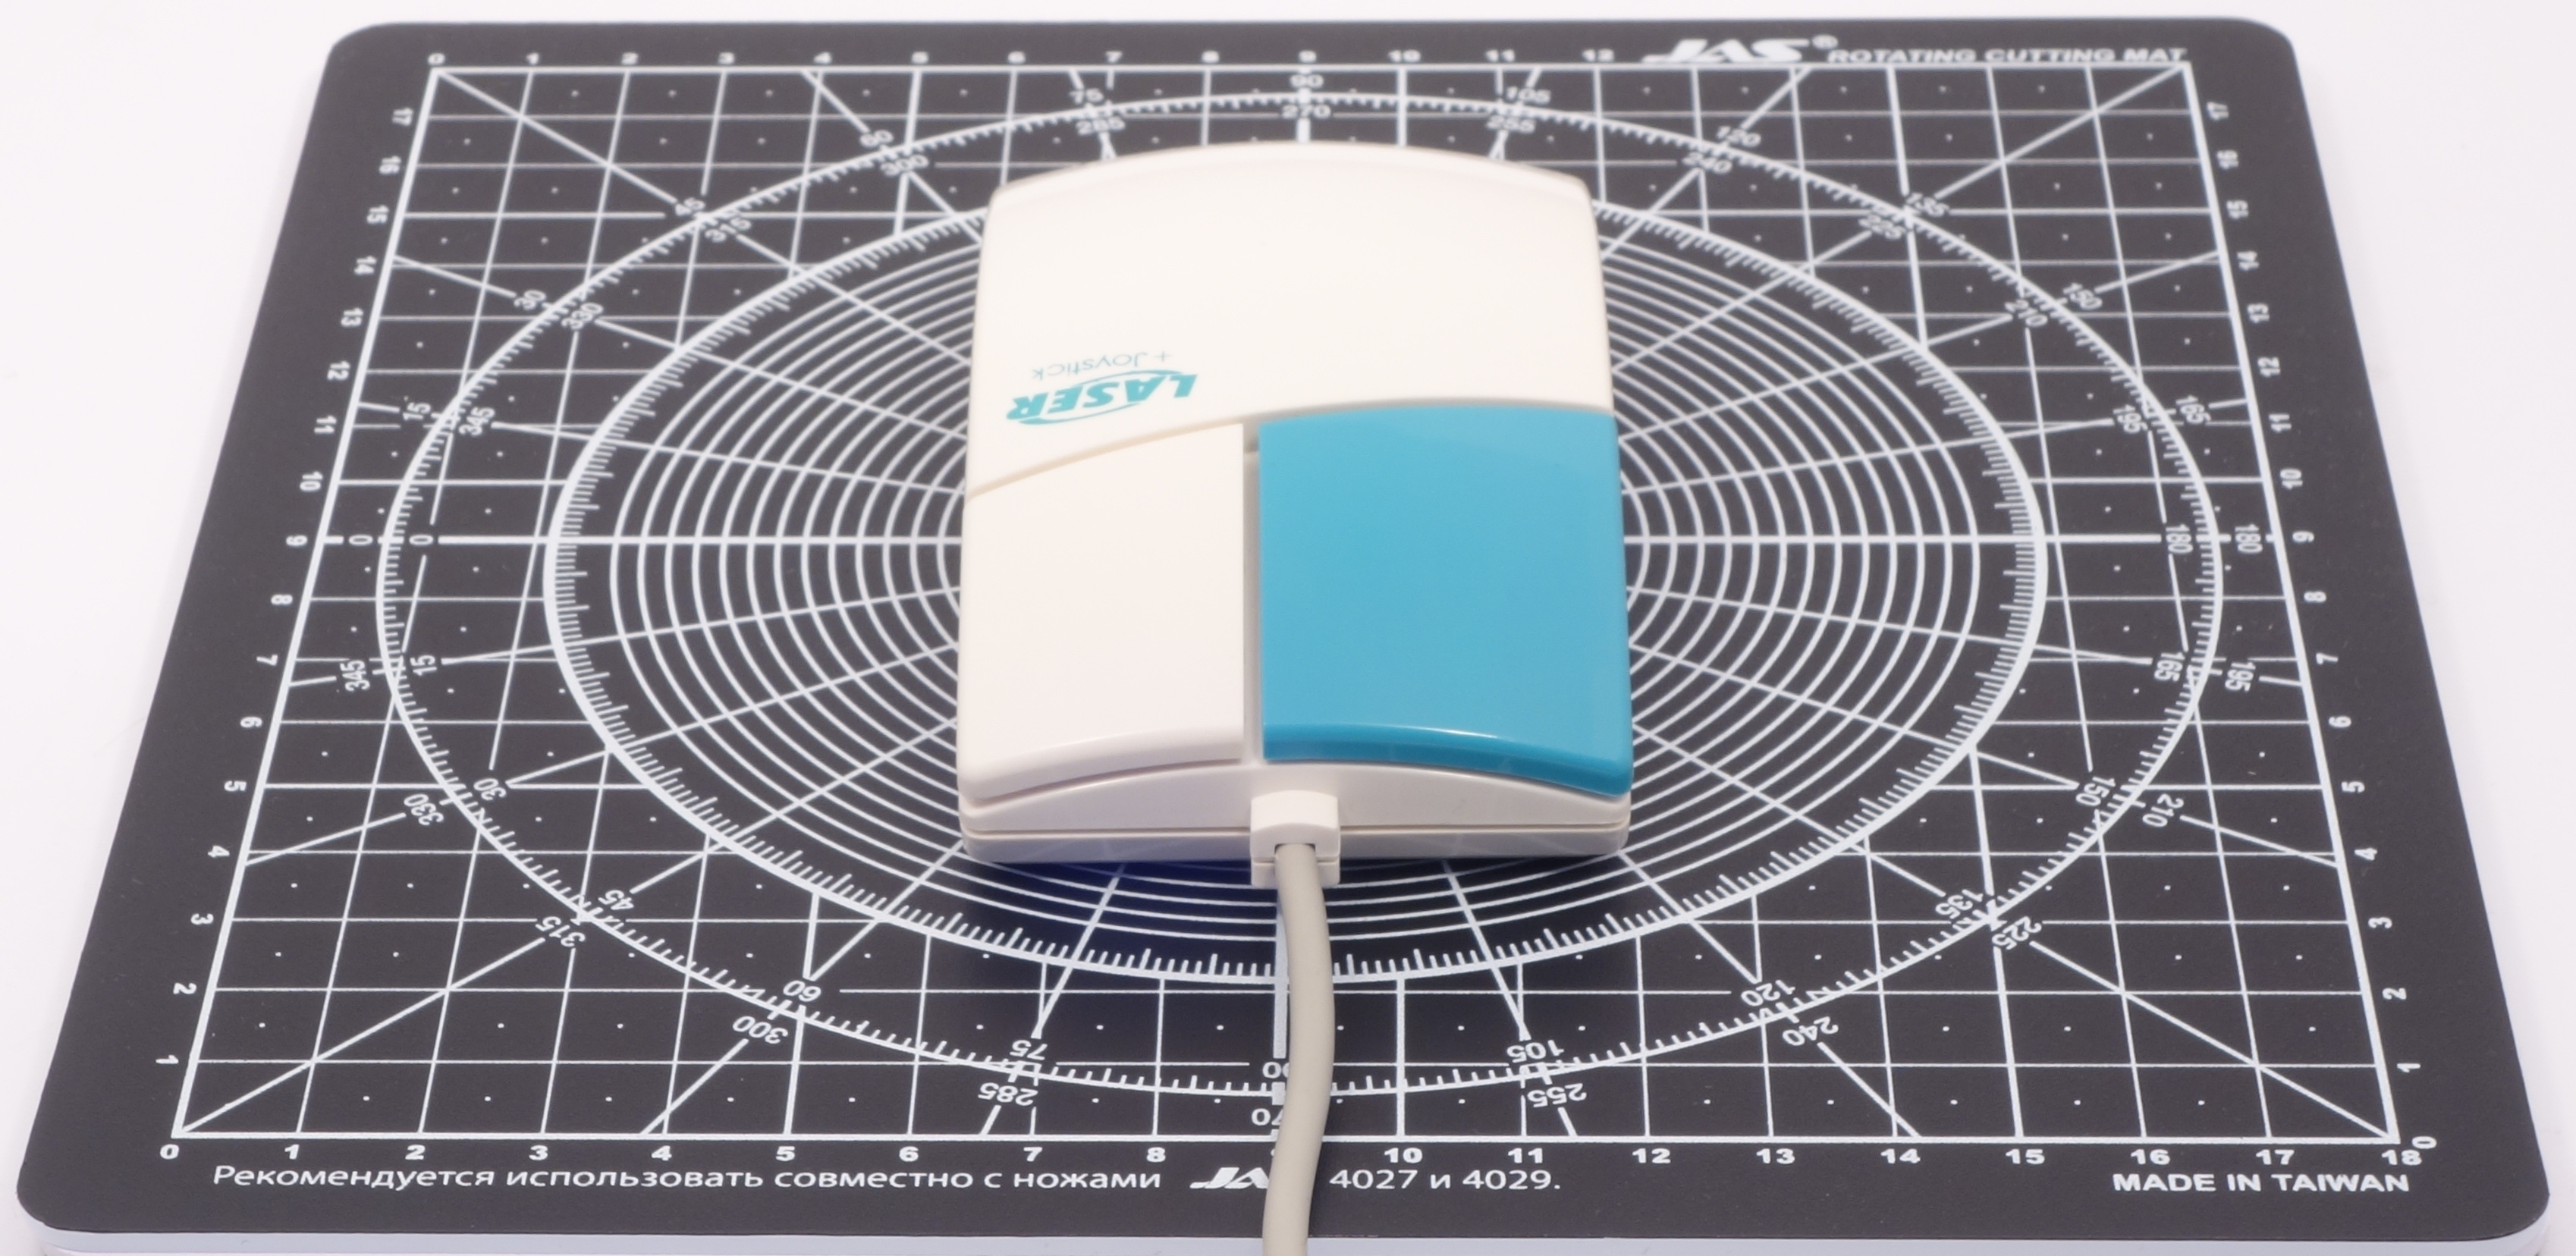
\includegraphics[scale=0.3]{1996_hi-bon_laser_mouse/size.jpg}
    \caption{Hi-Bon Optical laser mouse на размерном коврике с шагом сетки 1~см}
    \label{fig:OpticalLaserMouseSize}
\end{figure}

Третья кнопка, достаточно удобно расположенная сбоку корпуса в зоне досягаемости большого пальца (рис. \ref{fig:OpticalLaserMouseHand}) используется для переключения режимов. Дополнительно эта боковая кнопка эмулирует двойное нажатие, однако учитывая ее малую площадь (в отличие от основных двух), данная функция не слишком удобна для частого использования.

\begin{figure}[h]
    \centering
    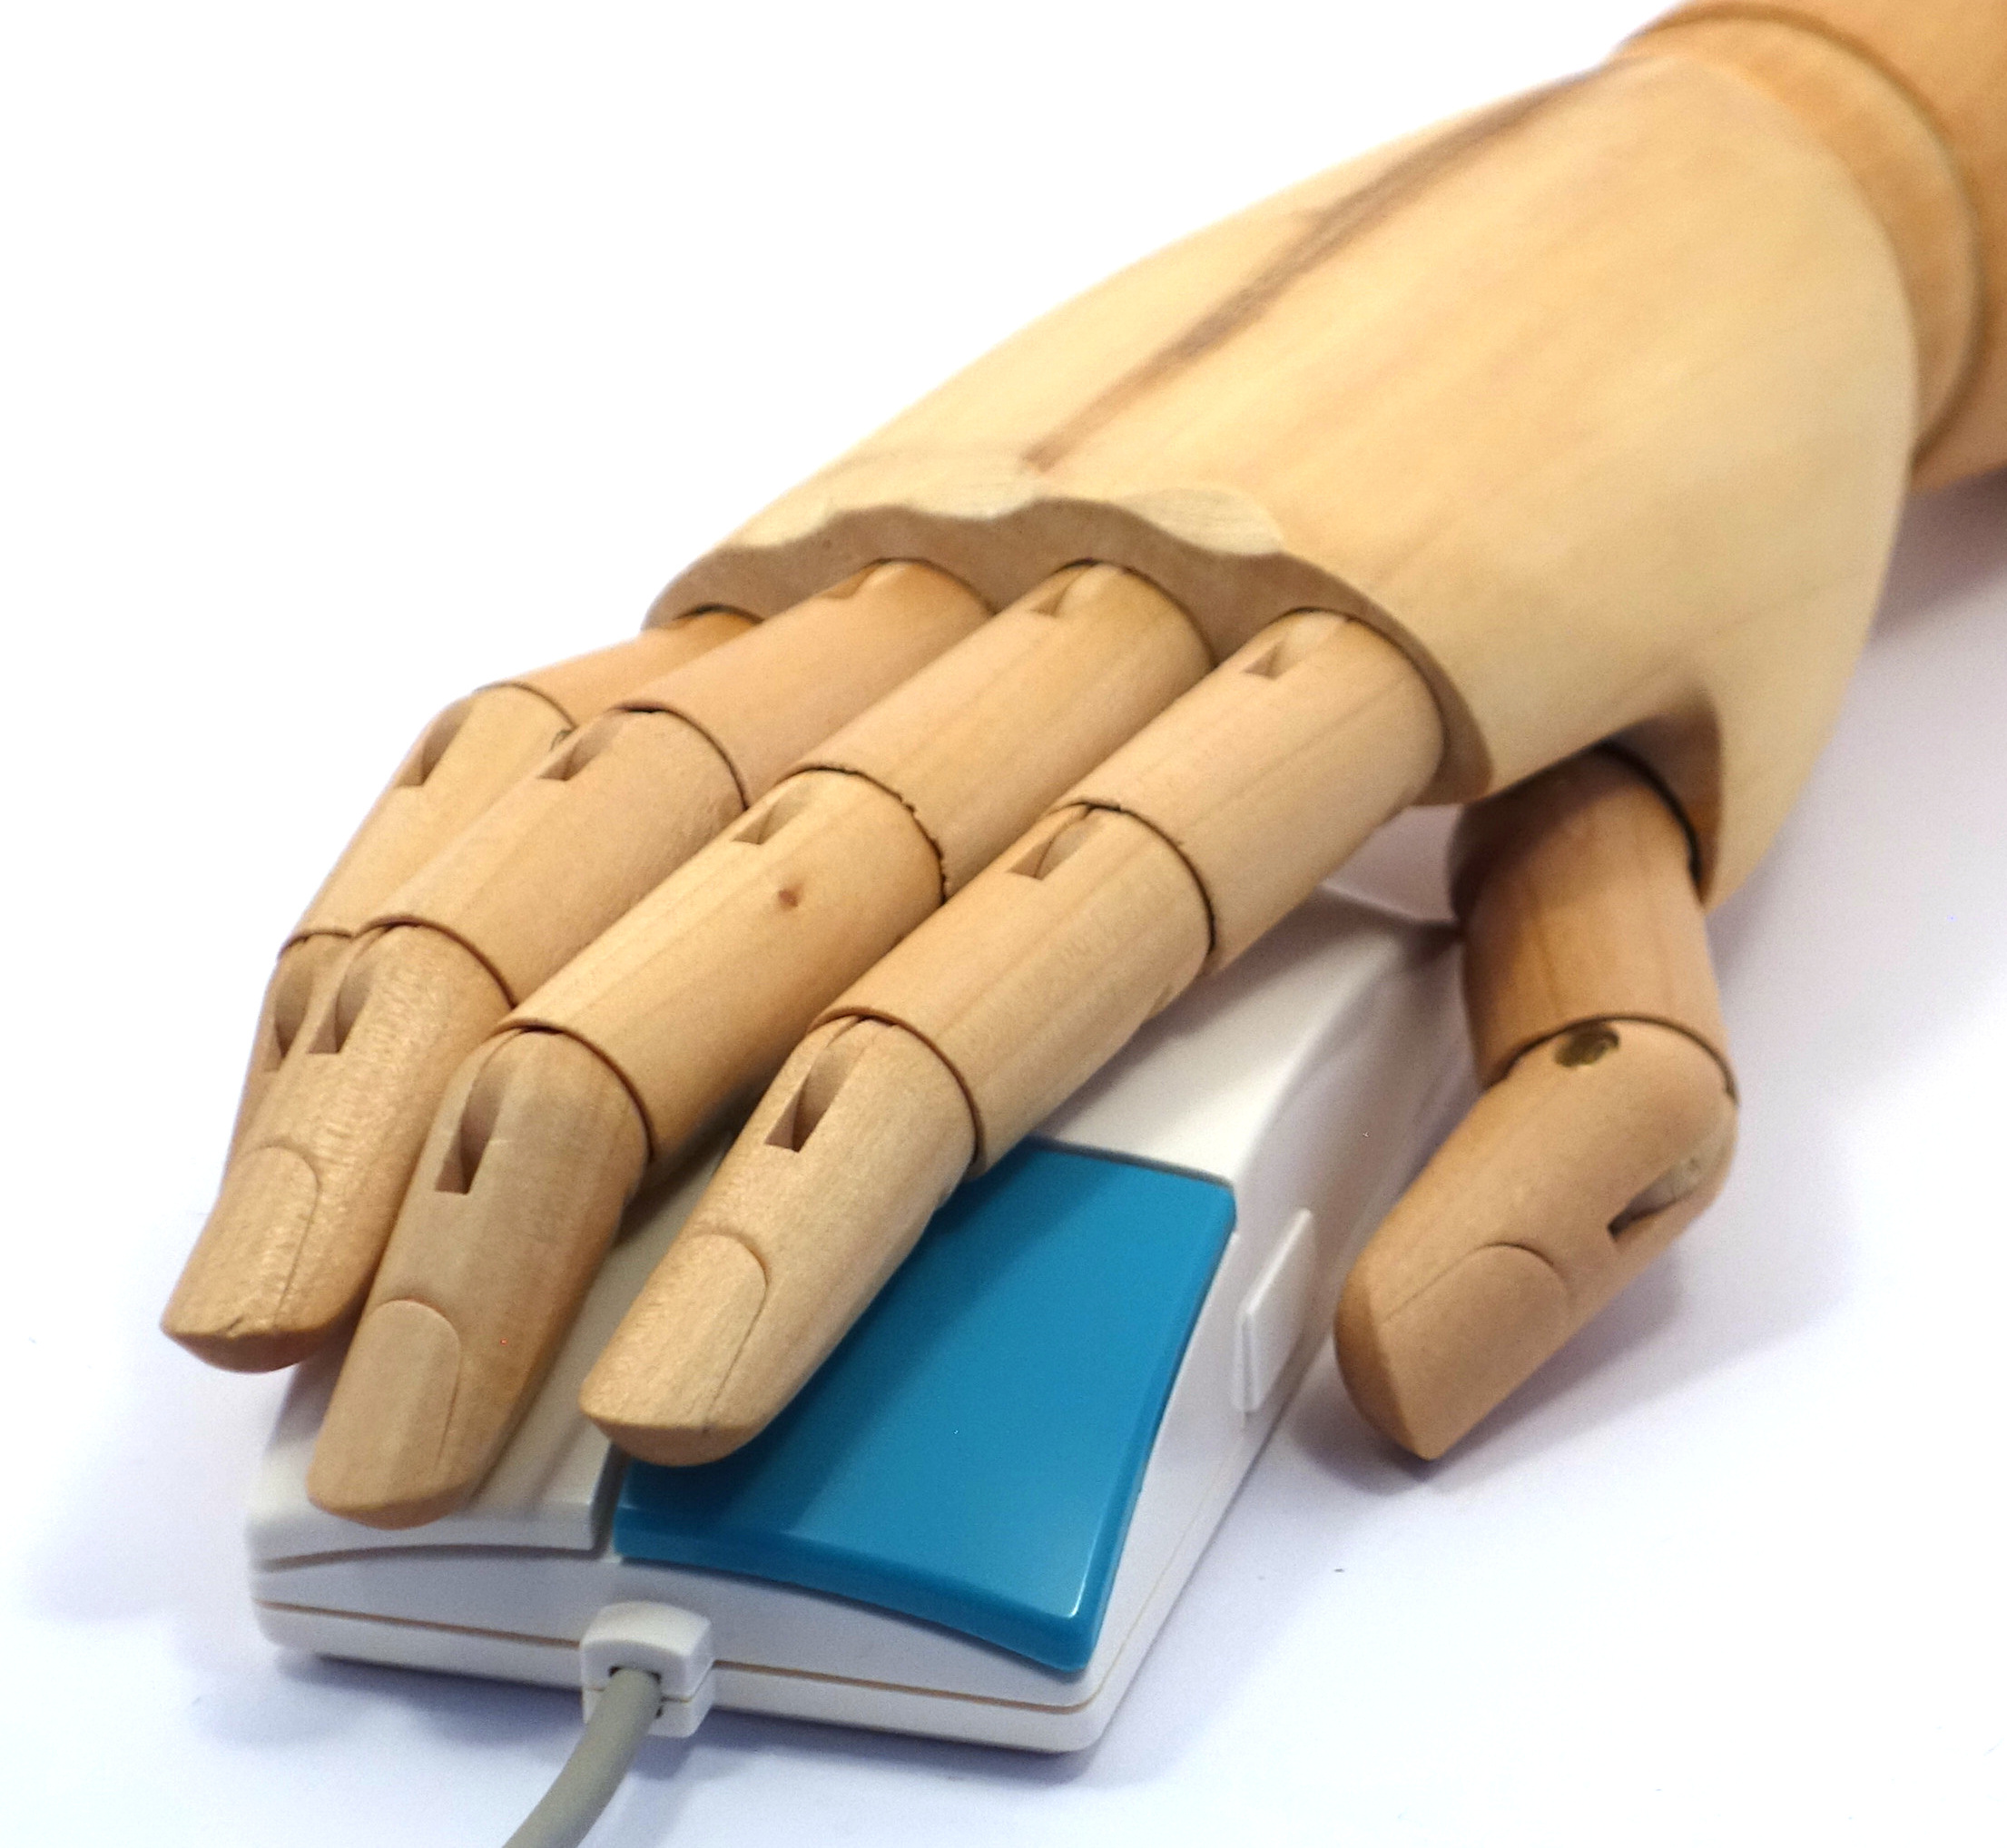
\includegraphics[scale=0.3]{1996_hi-bon_laser_mouse/hand_60.jpg}
    \caption{Изображение Hi-Bon Optical laser mouse с моделью руки человека}
    \label{fig:OpticalLaserMouseHand}
\end{figure}

Laser mouse содержит управляющий микроконтроллер, реализующий 3 режима работы.

Первый режим "--- стандартный. Второй (включается одновременным нажатием дополнительной кнопки сбоку корпуса и левой кнопки мыши) переключает мышь в режим джойстика. В этом режиме перемещение мыши от центра (точки, в которой мышь находилась в момент переключения режима) интерпретируется как отклонение рукоятки джойстика. Необходимо заметить, что применение мыши в качестве игрового джойстика является достаточно неудобным \cite{LittleMagick}, учитывая что центр, к которому необходимо вернуться чтобы остановить движение персонажа, никак не обозначен.

Третий режим (включается одновременным нажатием боковой и правой кнопок) активирует т.~н. «прецизионный» режим работы, предназначенный для художников и дизайнеров (фактически, активирует заявленное разрешение 450 DPI).

Внутреннее устройство (рис. \ref{fig:OpticalLaserMouseInside}) показывает два пучка световодов, расходящиеся по четырем фотоприемникам. Применение удвоенного числа фотоприемников позволило разработчикам отказаться от расчерчивания коврика продольными и поперечными полосами (в отличие от более дешевой модели Q500 и оптических мышей Mouse Systems), заменив их сеткой темных точек. Благодаря этому поворот коврика на $90^\circ$ не влияет на работоспособность мыши; однако углы некратные 90 затрудняют считывание движения, а угол $45^\circ$ делает управление курсором практически невозможным \cite{comparison}.

\begin{figure}[h]
    \centering
    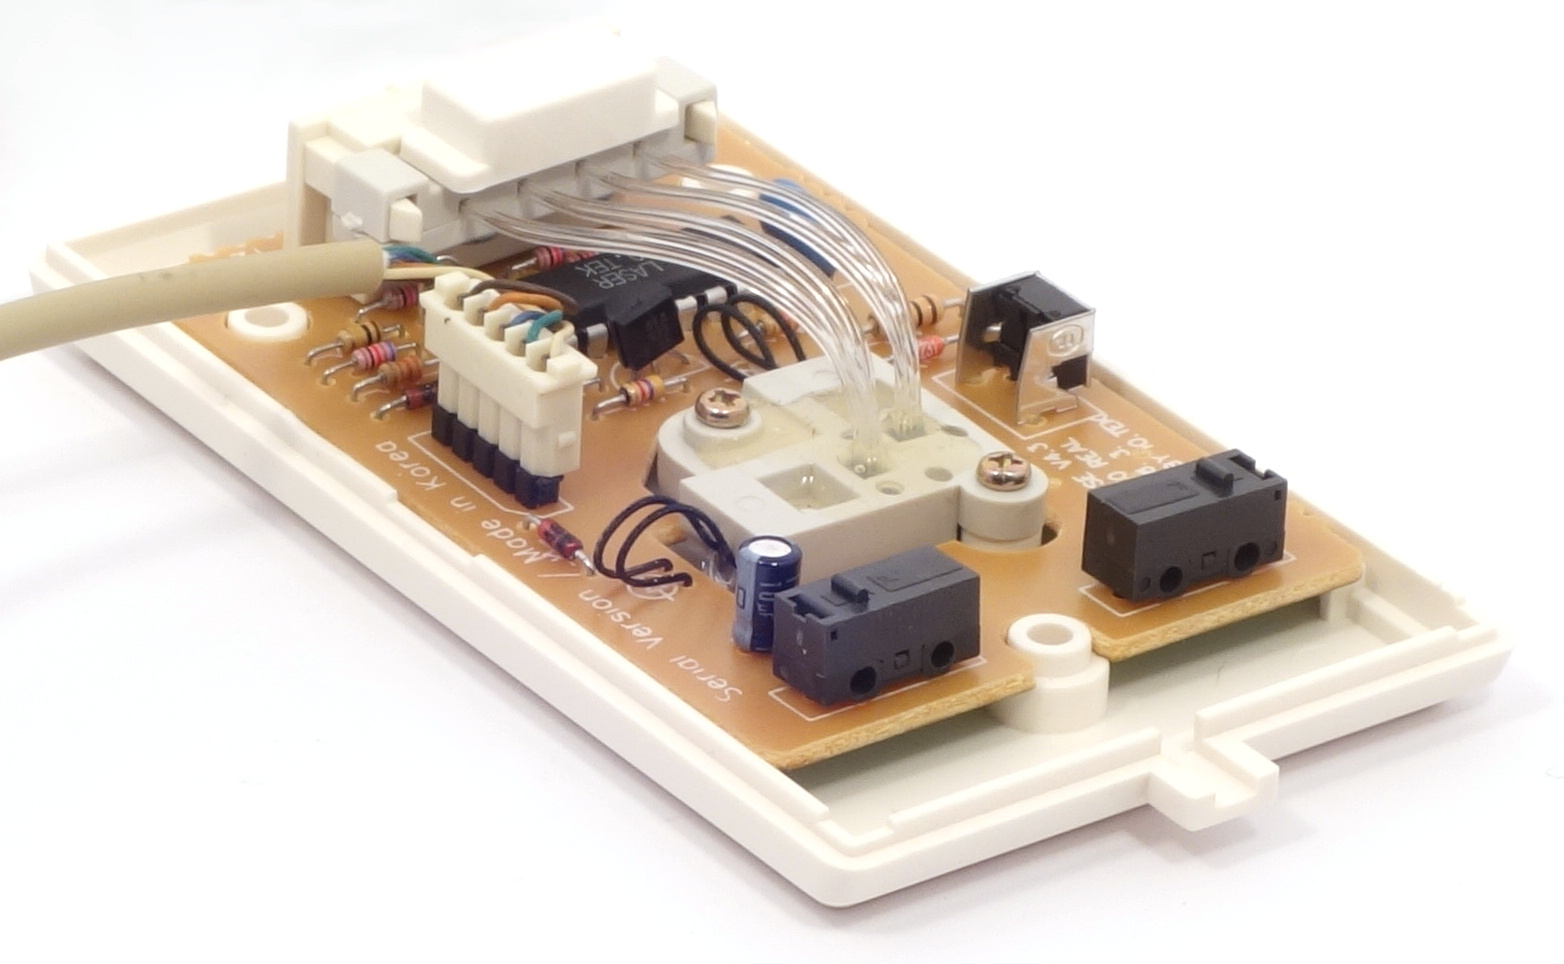
\includegraphics[scale=0.8]{1996_hi-bon_laser_mouse/inside_60.jpg}
    \caption{Hi-Bon Optical laser mouse в разобранном виде}
    \label{fig:OpticalLaserMouseInside}
\end{figure}

Надпись на печатной плате показывает, что данная мышь была, как и мышь Q500, разработана на контрактной основе компанией iO TEK в 1996 году.

\begin{thebibliography}{9}
\bibitem{LittleMagick} This Serial ''Optical Laser Mouse'' from 1996 \url{https://www.youtube.com/watch?v=8CeKiSn5lGU}
\bibitem{comparison} LMOX2, The Other Weirdest Mouse \url{https://www.youtube.com/watch?v=2UXmDuiqMW0}

\end{thebibliography}
\end{document}
